%\part{Spezifikation}

\chapter{Kapitel}

Im Folgenden werden die Use-Case-Diagramme des Sech-Browsers übersichtlich vorgestellt. Diese veranschaulicht alle verschiedenen Funktionalitäten, die der Benutzer tätigen kann.

\section{Menüführung des Browsers Teil 1}

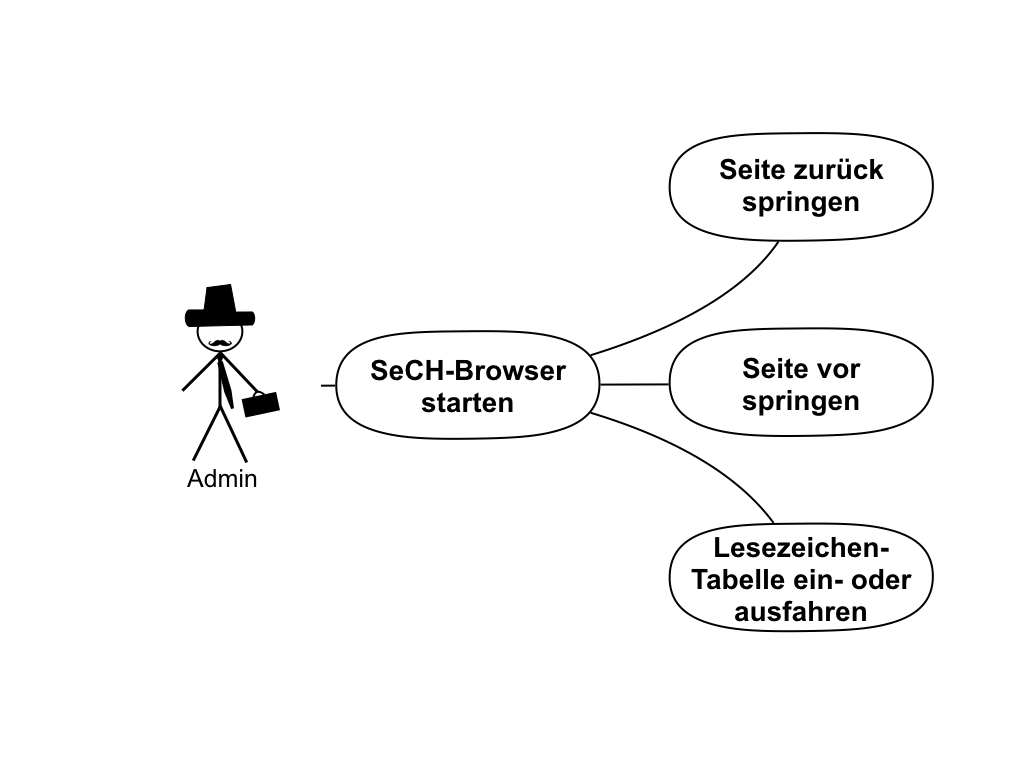
\includegraphics[width=\textwidth]{Use-Case-Diagramme.001.png}
	\caption{Use-Case-Diagramm - Menüführung Teil 1}
	\label{fig:Menüführung Teil 1}
	
Dieses Use-Case Diagramm zeigt die wesentlichen Funktionen des Browsers an. Der Nutzer kann auf einer Homepage eine Seite zurück- und vorspringen. Weiterhin hat er die Möglichkeit die Lesezeichen-Tabelle auszufahren und im Anschluss diese wieder einzufahren.

\section{Lesezeichenverwaltung des Browsers}

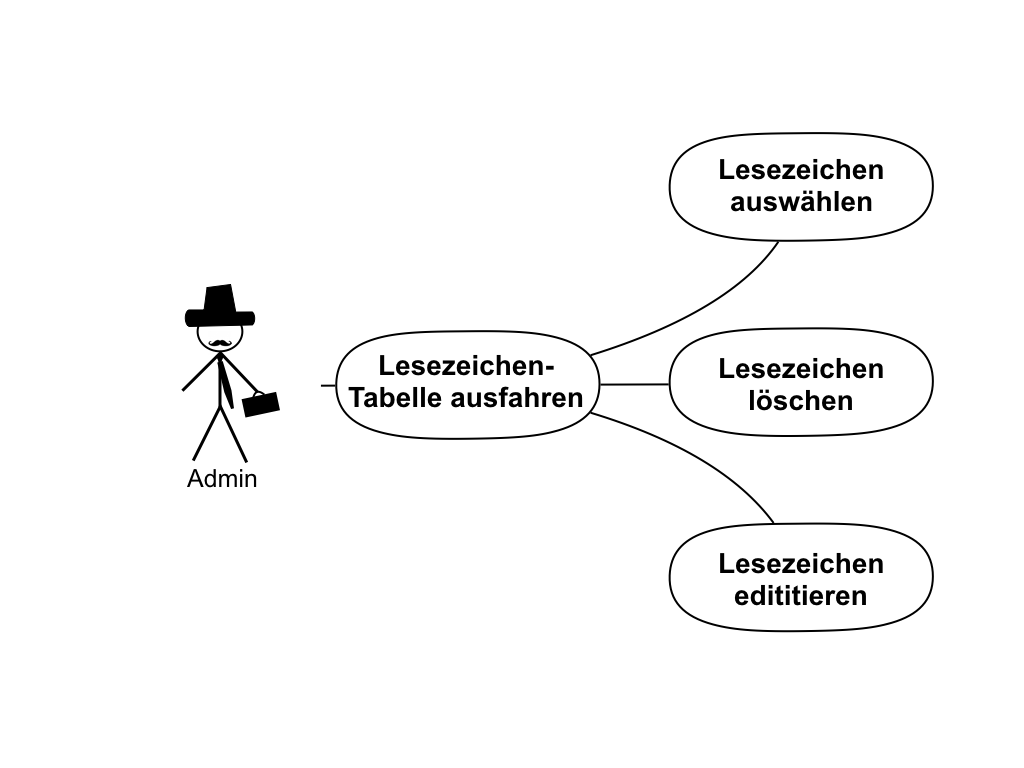
\includegraphics[width=\textwidth]{Use-Case-Diagramme.002.png}
	\caption{Use-Case-Diagramm - Lesezeichenverwaltung}
	\label{fig:Lesezeichenverwaltung}

Ist die Lesezeichen-Tabelle ausgefahren, so kann der Benutzer ein persönlich angelegtes Lesezeichen anklicken und es wird die von ihm gewünschte Seite geladen. Das Löschen und das Editieren, ausgewählter Lesezeichen, ist ebenfalls in der Tabelle verwirklichbar.

\section{Menüführung des Browsers Teil 2}

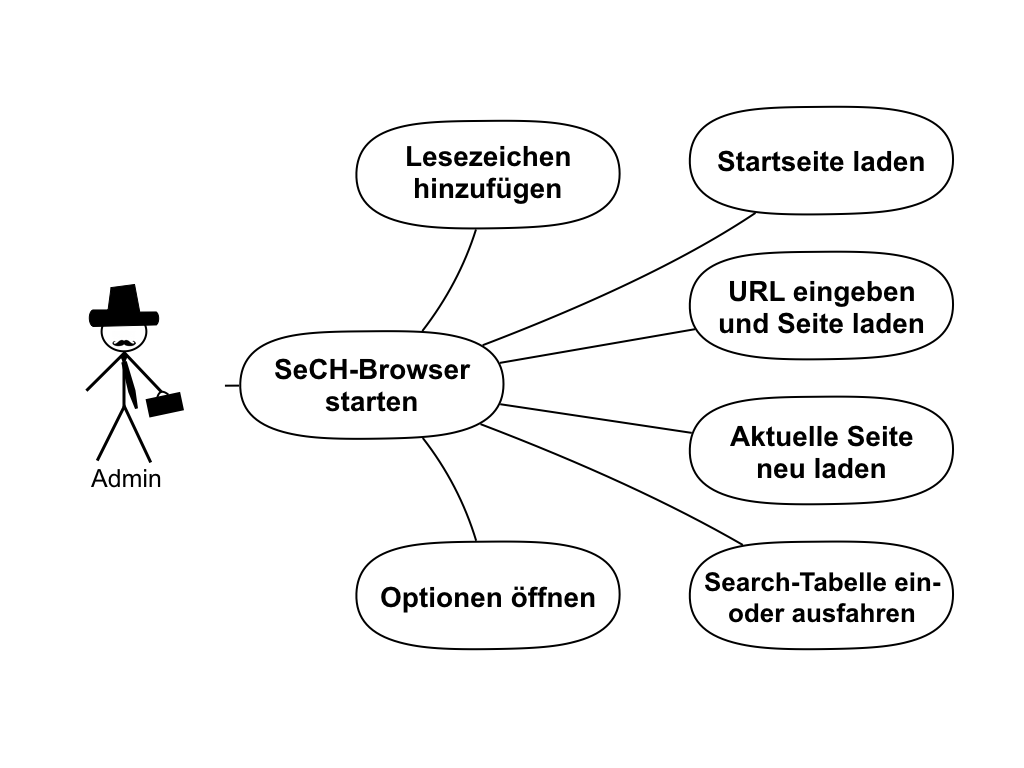
\includegraphics[width=\textwidth]{Use-Case-Diagramme.003.png}
	\caption{Use-Case-Diagramm - Menüführung Teil 2}
	\label{fig:Menüführung Teil 2}

In diesem Use-Case Diagramm werden weitere Navigationselemente des Browsers vorgestellt. Der Nutzer kann eigene Lesezeichen hinzufügen, die von ihm definierte Startseite laden, eine URL in die Address-Bar eingeben und diese dann laden, die aktuelle Seite neu laden, die Search-Tabelle aus- und einzufahren und das Fenster für Optionen öffnen.

\section{Search-Tagverwaltung des Browsers}

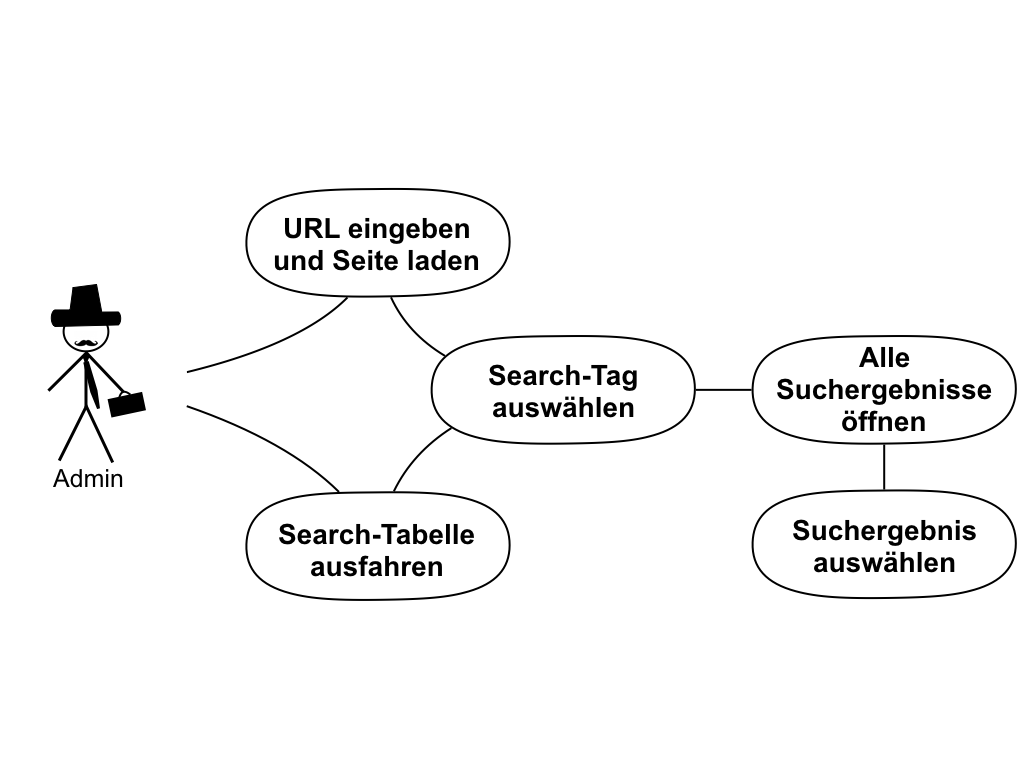
\includegraphics[width=\textwidth]{Use-Case-Diagramme.004.png}
	\caption{Use-Case-Diagramm - Search-Tagverwaltung}
	\label{fig:Search-Tagverwaltung}

Der Nutzer kann durch zwei verschiedene Wege Suchergebnisse für das gewünschte Search-Tag anzeigen lassen. Zunächst muss der Nutzer durch Eingabe und Bestätigung einer URL die Seite aufrufen. Erste Variante ist das gewünschte Search-Tag, welches hervorgehoben wird, anzuklicken. Zweite Variante ist durch Ausfahren der Search-Tabelle das gewünschte Search-Tag auszuwählen. Beide Wege führen zum selben Ergebnis, und zwar die Anzeige des ersten Suchergebnisses des jeweiligen Search-Tags. Zusätzlich kann der Nutzer alle weitere Suchergebnisse zu einem Search-Tag anzeigen lassen.

\section{Browser-Einstellungen}

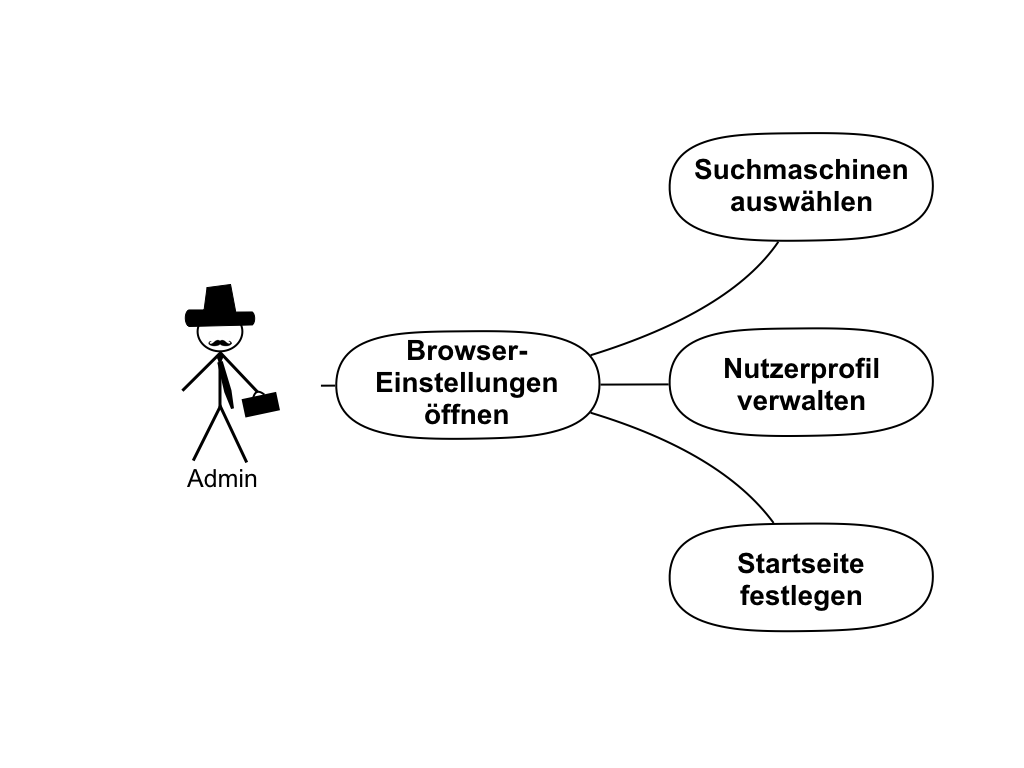
\includegraphics[width=\textwidth]{Use-Case-Diagramme.005.png}
	\caption{Use-Case-Diagramm - Browser-Einstellungen}
	\label{fig:Browser-Einstellungen}

Befindet sich der Nutzer in den Browser-Einstellungen, so hat er die Möglichkeit bestimmte Suchmaschinen, welche für die Suchergebnisse der Search-Tags verwendet werden, zu aktivieren oder diese zu deaktivieren. Im Weiteren kann der Benutzer sein persönliches Nutzerprofil verwalten und seine Startseite für die Applikation festlegen, welche direkt nach dem Öffnen der Anwendung als erste Seite geladen wird.
